
\usetikzlibrary{positioning, shapes, trees, graphs} % RNA trees
\newcommand{\scale}{0.6}

\chapter{Uvod a motivace}

\section{TODO - uvod}
%TODO


\section{Reprezentacia sekundarnej struktury}

Definicia \ref{def:RNA_sekundarna_struktura} nam ponuka reprezentovat sekundarnu strukturu
ako usporiadany strom.

\begin{figure}[H]
\centering
%TODO: vlastny obrazok... namiesto clankoveho
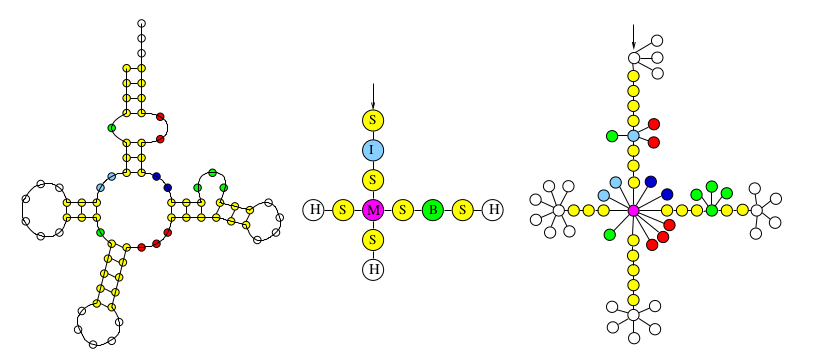
\includegraphics[width=130mm, height=70mm]{../img/stromova_reprezentacia_rna.png}
\caption{Varianty reprezentacie vrcholov}
\label{obr:RNA_vrcholy}
\end{figure}

\begin{definice}\label{def:strom}
	Usporiadany zakoreneny strom je orientovany graf, v ktorom plati, ze hrany su orientovane
	vzdy v smere z predka na potomka. Okrem korena ma kazdy vrchol svojho predka.
  Naviac tu existuje usporiadanie medzi potomkami.
	\\
	Usporiadany les je usporiadana mnozina stromov.
	%TODO: obrazok usporiadania stromov
\end{definice}

Bez ujmy na obecnosti budeme o RNA hovorit ako o strome, aj ked sa moze stat, ze
struktura nebude celistva (teda nieje to strom, ale les). V tom pripade ale
iba pripojime korenovy vrchol, ktoreho potomkovia budu dane stromy.

Kazdy vrchol stromu moze reprezentovat napriklad motiv v strukture RNA, nukleotid, alebo bazovy par
Priklady mozno vidiet na obrazku \ref{obr:RNA_vrcholy}.

V nasej praci vrchol stromu reprezentuje bazovy par (vnutorny vrchol) a nesparovanu bazu (list stromu).
Strukturu do ktorej patri si totiz vieme lahko zistit z potomkov vrcholu.

%rna, from 5' to 3':
% AUGCAAACUGGCACCCUCAU
% (((((...))(...))..))

\begin{center}
  \begin{minipage}{.500\textwidth}
    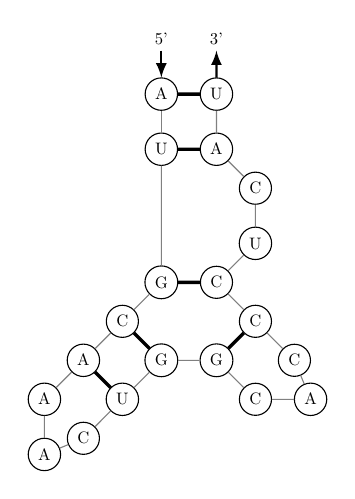
\begin{tikzpicture}[
        on grid,
        node distance = 0.7,
        -latex,
        scale = \scale,
        every node/.style = {scale = \scale},
        base/.style = {circle, draw},
        ends/.style = {draw = none, fill = none}]

      %ends, 5' a 3'
      \node[ends] (5end) {5'};
      \node[ends] (3end) [right = of 5end] {3'};

      %stem
      \node[base] (StemLeft1) [below = of 5end] {A};
      \node[base] (StemRight1) [right = of StemLeft1] {U};
      \node[base] (StemLeft2) [below = of StemLeft1] {U};
      \node[base] (StemRight2) [right = of StemLeft2] {A};

      %bulge
      \node[base] (Bulge1) [below right = of StemRight2] {C};
      \node[base] (Bulge2) [below = of Bulge1] {U};

      %stem
      \node[base] (StemRight3) [below left = of Bulge2] {C};
      \node[base] (StemLeft3) [left = of StemRight3] {G};

      %left-branch
      \node[base] (LBranchLStem1) [below left = of StemLeft3] {C};
      \node[base] (LBranchRStem1) [below right = of LBranchLStem1] {G};
      \node[base] (LBranchLStem2) [below left = of LBranchLStem1] {A};
      \node[base] (LBranchRStem2) [below left = of LBranchRStem1] {U};

      %left-branch-hairpin
      \node[base] (LBranchHairpin1) [below left = of LBranchLStem2] {A};
      \node[base] (LBranchHairpin2) [below = of LBranchHairpin1] {A};
      \node[base] (LBranchHairpin3) [below left = of LBranchRStem2] {C};

      %right-branch
      \node[base] (RBranchRStem1) [below right = of StemRight3] {C};
      \node[base] (RBranchLStem1) [below left = of RBranchRStem1] {G};

      %right-branch-hairpin
      \node[base] (RBranchHairpin1) [below right = of RBranchLStem1] {C};
      \node[base] (RBranchHairpin2) [right = of RBranchHairpin1] {A};
      \node[base] (RBranchHairpin3) [below right = of RBranchRStem1] {C};

      \begin{scope}[-]
      %pair edges
        \path[very thick]
        (StemLeft1) edge (StemRight1)
        (StemLeft2) edge (StemRight2)
        (StemLeft3) edge (StemRight3)
        (LBranchLStem1) edge (LBranchRStem1)
        (LBranchLStem2) edge (LBranchRStem2)
        (RBranchLStem1) edge (RBranchRStem1)
        ;
      %lines around molecule
        \path[color = gray]
        (StemLeft1) edge (StemLeft2)
        (StemLeft2) edge (StemLeft3)
        (StemLeft3) edge (LBranchLStem1)
        (LBranchLStem1) edge (LBranchLStem2)
        (LBranchLStem2) edge (LBranchHairpin1)
        (LBranchHairpin1) edge (LBranchHairpin2)
        (LBranchHairpin2) edge (LBranchHairpin3)
        (LBranchHairpin3) edge (LBranchRStem2)
        (LBranchRStem2) edge (LBranchRStem1)
        (LBranchRStem1) edge (RBranchLStem1)
        (RBranchLStem1) edge (RBranchHairpin1)
        (RBranchHairpin1) edge (RBranchHairpin2)
        (RBranchHairpin2) edge (RBranchHairpin3)
        (RBranchHairpin3) edge (RBranchRStem1)
        (RBranchRStem1) edge (StemRight3)
        (StemRight3) edge (Bulge2)
        (Bulge2) edge (Bulge1)
        (Bulge1) edge (StemRight2)
        (StemRight2) edge (StemRight1)
        ;
      \end{scope}

      \begin{scope}
        % edges to ends
        \path[thick]
        (5end) edge (StemLeft1)
        (StemRight1) edge (3end)
        ;
      \end{scope}
    \end{tikzpicture}
      %\caption{Molekula RNA}
      %\label{obr:RNA_rna}
  \end{minipage}
  \begin{minipage}{.450\textwidth}
    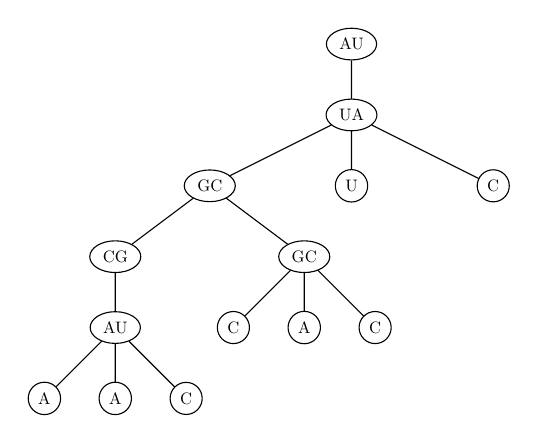
\begin{tikzpicture}[
        baseline,
        level distance = 1.5 cm,
        scale = \scale,
        every node/.style = {scale = \scale},
        basepair/.style = {ellipse, draw, minimum height = 0.3 cm, minimum width = 0.7 cm},
        unpaired/.style = {circle, draw, minimum width = 0.3 cm},
        level 2/.style = {sibling distance = 3 cm},
        level 3/.style = {sibling distance = 4 cm},
        level 4/.style = {sibling distance = 1.5 cm}
      ]
      \node[basepair] {AU}
      child {
        node[basepair] {UA}
        child {
          node[basepair] {GC}
          child {
            node[basepair] {CG}
            child {
              node[basepair] {AU}
              child {
                node[unpaired] {A}
              }
              child {
                node[unpaired] {A}
              }
              child {
                node[unpaired] {C}
              }
            }
          }
          child {
            node[basepair] {GC}
            child {
              node[unpaired] {C}
            }
            child {
              node[unpaired] {A}
            }
            child {
              node[unpaired] {C}
            }
          }
        }
        child {
          node[unpaired] {U}
        }
        child {
          node[unpaired] {C}
        }
      }
      ;
    \end{tikzpicture}
      %\caption{Stromova reprezentacia RNA}
      %\label{obr:RNA_tree}
  \end{minipage}
\end{center}




\section{Algoritmus}



